% !Mode:: "TeX:DE:UTF-8:Main"
%
%
%JOURNAL CODE  SEE DOCUMENTATION

\documentclass[examplefnt,biber]{nowfnt} % creates the journal version, needs biber version
%wrapper for book and ebook are created automatically.

\usepackage[utf8]{inputenc}

\usepackage{amsmath,amssymb,amsfonts,latexsym,dsfont,xspace}

% a few definitions that are *not* needed in general:
\newcommand{\ie}{\emph{i.e.}}
\newcommand{\eg}{\emph{e.g.}}
\newcommand{\etc}{\emph{etc}}
\newcommand{\now}{\textsc{now}}

%ARTICLE TITLE
\title{My First Thesis}


%ARTICLE SUB-TITLE
\subtitle{Smart Things as Said by Me}


%AUTHORS FOR COVER PAGE
% separate authors by \and, item by \\
% Don't use verbatim or problematic symbols.
% _ in mail address should be entered as \_
% Pay attention to large mail-addresses ...

%if there are many author twocolumn mode can be activated.
%\booltrue{authortwocolumn} %SEE DOCUMENTATION
\maintitleauthorlist{
Daan van Stigt \\
Institute for Logic, Language and Computation (ILLC) \\
}

%BIBLIOGRAPHY FILE
\addbibresource{BIB.bib}

\usepackage{mwe}

% %AUTHORS FOR ABSTRACT PAGE
% \author[1]{Heezemans,Alet}
% \author[2]{Casey,Mike}
%
% \affil[1]{now publishers, Inc.; alet.heezemans@nowpublishers.com}
% \affil[2]{now publishers, Inc.; mike.casey@nowpublishers.com}
%
% \articledatabox{\nowfntstandardcitation}

\begin{document}

\makeabstracttitle

\begin{abstract}
This is the best thesis. I have all the best words. Also, do check out my code. You will be blown away. Such wow. Much amazings.

\end{abstract}

\chapter{Inside and outside recursion for minimal span-based parser}
\label{c-intro} % a label for the chapter, to refer to it later

\section{Semiring formulation}
So yeah, the highlights are: an edge connects three nodes, a parent and two \textsc{children}, each node is a labelled \textsc{span}; you need to identify the scoring function for an edge, let’s call it $w(e)$,  in this case we have
\begin{align}
    w(e) = f(\textsc{head}(e)) \bigotimes_{c \in \textsc{children}(e)} g(\textsc{span}(c))
\end{align}
where $f$ and $g$ are parametric functions; then you can compute the Inside recursion for a node v
\begin{align}
    I(v) = \bigoplus_{e \in BS(v)} w(e) \otimes \bigotimes_{c \in \textsc{children}(e)} I(c)
\end{align}
where I’m using $BS(v)$ to denote the set of edges incoming to $v$; note that BS here basically enumerates the different ways to segment the string under $(i,j)$ into two adjacent parts and the different labels of each child \textsc{span} (let’s call these $a$ and $b$, each an element in the labelset $L$), thus we can write
\begin{align}
I(v=[i,j,l]) = \bigoplus_{ \substack{ e=[i,j,l,k,a,b]: \\ a \in L, \\ b \in L, \\ k \in \{i+1,...,j-1\} } } w(e) \otimes I([i,k,a]) \otimes I([k+1,j,b])
\end{align}
Now the key is to realise that $w(e)$ factorises and therefore we can rewrite this as
\begin{align}
    I(v=[i,j,l]) = f(i,j,l) &\otimes \bigoplus_{k=i+1}^{j-1} g(i,k) \otimes g(k+1,j) \\
        &\otimes \bigoplus_{a \in L}  I([i,k,a]) \\
        &\otimes \bigoplus_{b\in L} I([k+1,j,b])
\end{align}
and this finally motivates having an inside table for the \textsc{span}s (with labels summed out), let’s call that
\begin{align}
    S(i,j) = \bigoplus_{l \in L} I(i,j,l)
\end{align}
and then we have the result
\begin{align}
\label{eq:inside-semiring}
    I(i,j,l) = f(i,j,l)\otimes \bigoplus_{k=i+1}^{j-1} g(i,k)\otimes g(k+1,j) \otimes S(i,k) \otimes S(k+1,j).
\end{align}


\section{Alternative formulation}

In this derivation we follow Michael Collins notes on the Inside-Outside Algorithm.\footnote{\url{http://www.cs.columbia.edu/~mcollins/io.pdf}}

Let a sentence be $x_1,\dots,x_n$, where each $x_i$
is a word. We are given a CFG $(N, \Sigma, R, S)$ in Chomsky normal
form. Let $\psi$ be a function that maps any rule production $r \in R$ of the form $\langle A \to B \;C, i, k, j \rangle$ or $\langle A, i, i+1 \rangle$ to a value $\psi(r) \geq 0$. Let a tree $T$ be a set of such rules $r$ with the only constraint that these rules make up a tree.

Following the minimal span parser we define $\psi$ as
\begin{align}
\label{eq:rule-score}
    \log\psi(A \to B \;C, i, k, j) &\triangleq s_{label}(i, j, A) + s_{span}(i, j) \\
    &\text{and} \\
    \log\psi(A, i, i+1) &\triangleq s_{label}(i, i+1, A) + s_{span}(i, i+1),
\end{align}
and thus the potential of a tree as
\begin{align}
\label{eq:tree-score}
    \log\Psi(T) &= \sum_{r \in T} \log\psi(r) \\
        &= \sum_{\langle A, i, j \rangle \in T} s_{label}(i, j, A) + s_{span}(i, j), \\
\end{align}
Note that the potential function as defined in \ref{eq:rule-score} disregards most of the information in a binary rule. In particular we see that $B$, $C$ and $k$, the labels and split-point of the children, are discarded.

Now note that equation \label{eq:tree-score} corresponds exactly to the second formula in section 3 of the minimal span-based parser paper
\begin{align}
s_{tree}(T) = \sum_{(\ell(i,j))\in T}[s_{label}(i, j, \ell) + s_{span}(i, j)] .
\end{align}
which is how I derived that \ref{eq:rule-score} is the correct formula for the rule score.

We obtain our CRF objective when we normalize this score globally
\begin{align}
\label{eq:crf-objective}
    P(T) &= \frac{\prod_{r \in T} \psi(r)}{\sum_{T' \in \mathcal{T}} \prod_{r' \in T'} \psi(r')} \\
\end{align}
or equivalently
\begin{align}
\label{eq:logcrf-objective}
    \log P(T) &= \sum_{r \in T} \log \psi(r) - \log \sum_{T \in \mathcal{T}} \prod_{r \in T} \psi(r) \\
\end{align}

From the aforementioned notes we get the following general result for the inside value $\alpha$. For all $A \in N$, for all $0 \leq i < n$
\begin{align}
    \label{eq:collins-inside}
    \alpha(A,i,i+1) = \psi(A, i, i+1)
\end{align}
and for all $(i, j)$ such that $1 \leq i < j \leq n$:
\begin{align}
    \label{eq:collins-inside}
    \alpha(A,i,j) = \sum_{A \to B C} \sum_{k=i+1}^{j-1} \psi(A \to B \;C, i, k, j) \cdot \alpha(B,i,k) \cdot \alpha(C,k,j)
\end{align}
% \begin{align}
% \label{eq:rule-score}
%     \log\psi(A \to B \;C, i, k, j) \triangleq s_{label}(i, j, A) + s_{span}(i, k) + s_{span}(k, j),
% \end{align}
Note that we are considering a CFG in which the rule set is complete, i.e.
\begin{align}
    \langle A \to B \;C \rangle \in R \text{ for each } (A, B, C) \in N^3,
\end{align}
and recall that the labels $B$ and $C$ do not appear in the scoring functions in \ref{eq:rule-score}. These facts will allow us to simplify the expression in formula \ref{eq:collins-inside} as
\begin{subequations}
\begin{align}
    \alpha(A,i,j) &= \sum_{B \in N} \sum_{C \in N} \sum_{k=i+1}^{j-1} \tilde{s}_{label}(i, j, A) \cdot \tilde{s}_{span}(i, j) \alpha(B,i,k) \cdot \alpha(C,k,j) \\
        &= \tilde{s}_{label}(i, j, A) \cdot \tilde{s}_{span}(i, j) \sum_{k=i+1}^{j-1} \sum_{B \in N} \alpha(B,i,k) \cdot \sum_{C \in N} \alpha(C,k,j) \\
        &= \tilde{s}_{label}(i, j, A) \cdot \tilde{s}_{span}(i, j) \sum_{k=i+1}^{j-1} S(i,k) \cdot S(k,j) \label{eq:final-inside}
\end{align}
\end{subequations}
where we've introduced a number of notational abbreviations
\begin{align}
    \tilde{s}_{label}(i, j, A) &= \exp( s_{label}(i, j, A) ) \\
    \tilde{s}_{span}(i, j) &= \exp( s_{span}(i, j) ) \\
    S(i,j) &= \sum_{A \in N} \alpha(A,i,j)
\end{align}
Note that this is the exact same formula as \ref{eq:inside-semiring}.

From equation \ref{eq:final-inside} we can deduce that we in fact do even need to store the values $\alpha(i, j, A)$ but that it suffices to only store the marginalized values $S(i, j)$. In this case, the recursion simplifies even further:
\begin{subequations}
\begin{align}
    S(i, j) &= \sum_{A \in N} \alpha(A,i,j) \\
        &=  \sum_{A \in N} \tilde{s}_{label}(i, j, A) \cdot \tilde{s}_{span}(i, j) \sum_{k=i+1}^{j-1} S(i,k) \cdot S(k,j) \\
        &= \Bigg[ \sum_{A \in N} \tilde{s}_{label}(i, j, A) \cdot \tilde{s}_{span}(i, j) \Bigg] \Bigg[\sum_{k=i+1}^{j-1} S(i,k) \cdot  S(k,j) \Bigg]
\end{align}
\end{subequations}
where we put explicit brackets to emphasize that independence of the subproblems of labeling and splitting. We can now recognize this as the `inside' equivalent of the expression from the paper\footnote{I believe there is actually an error in this equation: it should read  $s_{label}(i, j, \ell) + s_{span}(i, j)$ instead of just $s_{label}(i, j, \ell)$. This is implied by the score for a single node, which is given by equation \ref{eq:rule-score}, taken directly from the paper.}
\begin{align}
    s_{best}(i, j) = \max_{\ell} [s_{label}(i, j, \ell)] + \max_{k}[ s_{split}(i, k, j)].
\end{align}
The recursions are the same; the semirings are different. The viterbi recursion given above is in the \textsc{ViterbiSemiring}, which uses the $\max$ operator as $\oplus$; the inside recursion given in \ref{eq:final-inside} has standard addition (+) instead.


\section{Outside}
\begin{align*}
    \beta(A, i, j) &= \sum_{B \to C A \in R} \sum_{k=1}^{i-1} \psi(B \to C A, k, i-1, j) \cdot \alpha(C, k, i-1) \cdot \beta(B, k, j) \\
            &\qquad + \sum_{B \to A C \in R} \sum_{k=j+1}^{n} \psi(B \to A, C, i, j, k) \cdot \alpha(C, j+1, k) \cdot \beta(B, i, k) \\
        &= \sum_{B \in N} \sum_{C \in N} \sum_{k=1}^{i-1} \psi(B, k, j) \cdot \alpha(C, k, i-1) \cdot \beta(B, k, j) \\
            &\qquad + \sum_{B \in N} \sum_{C \in N} \sum_{k=j+1}^{n} \psi(B, i, k) \cdot \alpha(C, j+1, k) \cdot \beta(B, i, k) \\
        &=  \sum_{k=1}^{i-1}  \Bigg[ \sum_{B \in N} \psi(B, k, j)  \cdot \beta(B, k, j) \Bigg] \cdot \Bigg[ \sum_{C \in N} \alpha(C, k, i-1) \Bigg] \\
            &\qquad + \sum_{k=j+1}^{n}  \Bigg[ \sum_{B \in N}  \psi(B, i, k) \cdot \beta(B, i, k) \Bigg] \cdot  \Bigg[ \sum_{C \in N} \alpha(C, j+1, k) \Bigg] \\
        &=  \sum_{k=1}^{i-1}  S'(k, j) \cdot S(k, i-1) + \sum_{k=j+1}^{n} S'(i, k) \cdot  S(j+1, k) \\
\end{align*}
where
\begin{align*}
    S(i, j) &= \sum_{A \in N} \alpha(A, i, j) \\
    S'(i, j) &= \sum_{A \in N} \psi(A, i, j) \beta(A, i, j)
\end{align*}


\chapter{Semisupervised learning}

Throughout these note we write $x$ for a sentence, $y$ for a (latent) constituency tree, and $\mathcal{Y}(x)$ for the \textit{yield} of $x$, that is, all trees that can be assigned to $x$. Furthermore, let $\mathbb{L}$ be a set of pairs $(x, y)$ of sentences with gold trees, and let $\mathbb{U}$ be a set of unlabeled sentences $x$.

We define the following semi-supervised objective
\begin{align}
    \mathcal{J} \triangleq \mathcal{J}_{\mathcal{S}} + \alpha \mathcal{J}_{\mathcal{U}},
\end{align}
were $\mathcal{J}_{\mathcal{S}}$ is the supervised objective optimized over $\mathbb{L}$ and $\mathcal{J}_{\mathcal{U}}$ the unsupervised objective optimized over $\mathbb{U}$. We introduce $\alpha \in \mathbb{R}$ as an arbitrary scalar controlling the contribution of the unsupervised objective.

\section{Supervised objective}
Let $p_{\theta}(x,y)$ be parametrized by a Generative RNNG \citep{Dyer+2016:RNNG}. Then our supervised objective is
\begin{align}
    \mathcal{J}_{\mathcal{S}}
        &\triangleq \sum_{(x,y) \in \mathbb{L}} \log p_{\theta} (x, y) \\
\end{align}
This objective is optimized as usual using stochastic gradient estimates:
\begin{align}
    \nabla_{\theta} \mathcal{J}_{\mathcal{S}}
        &\approx \frac{|\mathbb{L}|}{n} \sum_{i=1}^n \nabla_{\theta} \log p_{\theta} (x^{(i)}, y^{(i)}), \\
\end{align}
where $\{(x^{(i)}, y^{(i)})\}_{i=1}^n$ is a mini-batch sampled uniformly from $\mathbb{L}$. To compute $\nabla_{\theta} \log p_{\theta}(x^{(i)}, y^{(i)})$ we rely on automatic differentiation \citep{Baydin+2015:AD}.

\section{Unsupervised objective}
Consider the following objective to be maximized:
\begin{subequations}
\begin{align}
    \mathcal{J}_{\mathcal{U}}
        &\triangleq \sum_{x \in \mathbb{U}} \log p (x) \\
        &= \sum_{x \in \mathbb{U}} \log \sum_{y \in \mathcal{Y}(x)} p_{\theta}(x, y)
\end{align}
\end{subequations}
This is a language modelling objective, in which we treat $y$ as latent, and $p_{\theta}(x,y)$ is a generative RNNG. A consequence the independence assumptions of the RNNG (or better: lack thereof) is that the sum over trees $y$ is no longer tractable.  To optimize this objective we must fall back on approximate methods.

\paragraph{Variational approximation} We optimize the objective using variational inference \citep{Blei+2016:VI}. We introduce a posterior $q_{\lambda}(y|x)$ parametrised by $\lambda$ and use Jensen's inequality to derive a variational lower bound:
\begin{subequations}
\begin{align}
    \log p (x)
        &= \log \sum_{y \in \mathcal{Y}(x)} q_{\lambda}(y|x) \frac{p_{\theta}(x, y)}{q_{\lambda}(y|x)} \\
        &= \log \mathbb{E}_{q_{\lambda}} \bigg[\frac{p_{\theta}(x, y)}{ q_{\lambda}(y|x)} \bigg] \\
        &\geq \mathbb{E}_{q_{\lambda}} \bigg[\log \frac{p_{\theta}(x, y)}{q_{\lambda}(y|x)} \bigg] \\
        &= \mathbb{E}_{q_{\lambda}} \big[\log p_{\theta}(x, y)  - \log q_{\lambda}(y|x) \big] \triangleq \mathcal{L}(\theta, \lambda)
\end{align}
\end{subequations}
The only requirement for $q_{\lambda}$ is that
\begin{align}
    p(x,y) > 0 \Rightarrow q(y|x) > 0 \qquad \text{for all $x$ and $y \in \mathcal{Y}(x)$}.
\end{align}
Any discriminatively trained parser fulfills this requirement.

The lower bound $\mathcal{L}(\theta, \lambda)$ will be optimized by gradient optimization, which means we will need to take the gradients $\nabla_{\theta} \mathcal{L}(\theta, \lambda)$ and $\nabla_{\lambda} \mathcal{L}(\theta, \lambda)$.

\paragraph{Gradients of joint parameters} The first gradient is easy and permits a straightforward Monte-Carlo estimate:
\begin{subequations}
\begin{align}
    \nabla_{\theta} \mathcal{L}(\theta, \lambda)
        &= \nabla_{\theta} \mathbb{E}_{q_{\lambda}} \big[\log p_{\theta}(x, y)  - \log q_{\lambda}(y|x) \big] \\
        &= \mathbb{E}_{q_{\lambda}} \big[ \nabla_{\theta} \log p_{\theta}(x, y)  -  \nabla_{\theta} \log q_{\lambda}(y|x) \big] \\
        &= \mathbb{E}_{q_{\lambda}} \big[ \nabla_{\theta} \log p_{\theta}(x, y) \big] \\
        &\approx \frac{1}{n}\sum_{i=1}^n  \nabla_{\theta} \log p_{\theta}(x, y^{(i)})
\end{align}
\end{subequations}
where $y_i \sim q_{\lambda}(y|x)$ for $i=1,\dots,n$. We can move the gradient inside the expectation (second equality) because $q$ does not depend on $\theta$.

\paragraph{Gradients of posterior parameters}
The second gradient is harder and requires us to rewrite the objective:
\begin{subequations}
\begin{align}
\nabla_{\lambda} \mathcal{L}(\theta, \lambda)
        &= \nabla_{\lambda} \mathbb{E}_{q_{\lambda}} \big[\log p_{\theta}(x, y)  - \log q_{\lambda}(y|x) \big] \\
        &= \nabla_{\lambda} \sum_{y} \big\{ q_{\lambda}(y|x) \log p_{\theta}(x, y) - q_{\lambda}(y|x)\log q_{\lambda}(y|x) \big\} \\
        &= \sum_{y} \big\{ \nabla_{\lambda} q_{\lambda}(y|x) \log p_{\theta}(x, y) \\
        &\qquad\qquad - \nabla_{\lambda} q_{\lambda}(y|x)\log q_{\lambda}(y|x) \\
        &\qquad\qquad -  q_{\lambda}(y|x)\nabla_{\lambda}\log q_{\lambda}(y|x) \big\} \\
        &= \sum_{y} \big\{ \nabla_{\lambda} q_{\lambda}(y|x) \log p_{\theta}(x, y) - \nabla_{\lambda} q_{\lambda}(y|x)\log q_{\lambda}(y|x) \big\} \\
        &= \sum_{y} \big\{(\log p_{\theta}(x, y) - \log q_{\lambda}(y|x))\nabla_{\lambda} q_{\lambda}(y|x) \big\} \\
        &= \sum_{y} \big\{(\log p_{\theta}(x, y) - \log q_{\lambda}(y|x)) q_{\lambda}(y|x)\nabla_{\lambda} \log q_{\lambda}(y|x) \big\}   \\
        &= \mathbb{E}_{q_{\lambda}} \big[ (\log p_{\theta}(x, y) - \log q_{\lambda}(y|x))  \nabla_{\lambda} \log q_{\lambda}(y|x) \big\} \\
        &= \mathbb{E}_{q_{\lambda}} \big[ l(x, y) \nabla_{\lambda} \log q_{\lambda}(y|x) \big]
\end{align}
\end{subequations}
Where we've defined a learning signal $l(x, y) \triangleq \log p_{\theta}(x, y) - \log q_{\lambda}(y|x)$.

In this derivation we used the identity
\begin{align}
    \nabla_{\lambda}\log q_{\lambda}(y|x) &= \frac{\nabla_{\lambda} q_{\lambda}(y|x)}{q_{\lambda}(y|x)}
\end{align}
or equivalently
\begin{align}
    \nabla_{\lambda} q_{\lambda}(y|x) &= q_{\lambda}(y|x)\nabla_{\lambda}\log q_{\lambda}(y|x)
\end{align}
and the fact that
\begin{subequations}
\begin{align}
    \sum_{y} q_{\lambda}(y|x)\nabla_{\lambda}\log q_{\lambda}(y|x)
        &= \sum_{y}  q_{\lambda}(y|x) \frac{\nabla_{\lambda} q_{\lambda}(y|x)}{q_{\lambda}(y|x)}  \\
        &= \sum_{y} \nabla_{\lambda} q_{\lambda}(y|x) \\
        &= \nabla_{\lambda} \sum_{y} q_{\lambda}(y|x)\\
        &= \nabla_{\lambda} 1 \\
        &= 0. \\
\end{align}
\end{subequations}

This rewritten objective permits a straightforward MC estimate:
\begin{align}
\label{eq:score-function-estimator}
    \mathbb{E}_{q_{\lambda}} \big[ l(x,y) \nabla_{\lambda} \log q_{\lambda}(y|x) \big]
        &\approx \frac{1}{n}\sum_{i=1}^n  l(x,y^{(i)})\nabla_{\lambda} \log q_{\lambda}(x|y^{(i)})
\end{align}
where $y_i \sim q_{\lambda}(y|x)$ for $i=1,\dots,n$.

This estimator has been derived (in slightly different forms) in among others \citep{Williams1992:REINFORCE}, \citep{Paisley+2012:VISS}, \citep{Mnih+2014:NVIL}, \citep{Ranganath+2014:BBVI}, and \citep{Miao+16:LLVAE} and is known as the \textsc{reinforce} estimator \citep{Williams1992:REINFORCE}, or score function estimator (after the score function $\nabla_{\theta} \log p_{\theta}(x)$) \citep{Fu2006}.

\section{Optimization}
We use automatic differentiation \citep{Baydin+2015:AD} to obtain all our gradient estimates.

To get the gradients in formula \ref{eq:score-function-estimator} we rewrite it in the form of a surrogate objective \citep{Schulman+2015:surrogate}
\begin{align}
    L(\lambda) &= \frac{1}{n}\sum_{i=1}^n \log q_{\lambda}(x|y^{(i)}) \textsc{blockgrad}(l(x,y^{(i)}))
\end{align}
where \textsc{blockgrad} is function that `detaches' a parametrized function from the computation graph effectively turning it into a scalar. That is, loosely speaking
\begin{align}
    \textsc{blockgrad}(f_{\theta}(x)) &= f(x)
\end{align}
such that
\begin{align}
    \nabla_{\theta}\textsc{blockgrad}(f_{\theta}(x)) &= \nabla_{\theta} f(x) \\
        &= 0
\end{align}
Then differentiation of $L$ gives us the unbiased estimator
\begin{align}
    \nabla_{\lambda} L(\lambda) &= \frac{1}{n}\sum_{i=1}^n l(x,y^{(i)}) \nabla_{\lambda} \log q_{\lambda}(x|y^{(i)})
\end{align}

\section{Variance reduction}
We have derived an estimator for the gradient of the posterior parameters in the unsupervised objective. This estimator is unbiased, but is known to have high variance, often too much to be useful \citep{Paisley+2012:VISS}. Two effective methods to counter this are control variates and baselines \citep{Ross:2006:SIM}.

\paragraph{Variance of estimator} First, let's analyze the variance of our estimator. Note that our expectation is of the general form
\begin{align}
    \mu \triangleq \mathbb{E}\big[f(X)\big]
\end{align}
and that we estimate this quantity by generating $n$ independent samples $X_1,\dots,X_n \sim P(X)$ and computing
\begin{align}
    \hat{\mu} \triangleq \frac{1}{n} \sum_{i=1}^n f(X_i).
\end{align}
This is an unbiased estimator for $\mu$ with error
\begin{align}
    \text{MSE} = \mathbb{E}\big[(\mu - \hat{\mu})^2\big] &= \text{Var}[ \hat{\mu} ] = \frac{\text{Var}[ \hat{\mu} ]}{n},
\end{align}
which means that the error is of the order
\begin{align}
    \mu - \hat{\mu} \sim \sqrt{\frac{\text{Var}[ \hat{\mu} ]}{n}}
\end{align}
and reducing it linearly requires a quadratic number of samples.

In our particular case, the function $f$ is
\begin{align}
    f_{X=x}(Y) &\triangleq l(X,Y) \nabla_{\lambda} \log q_{\lambda}(Y|X=x)
\end{align}
where we have made explicit that $y$ is the random variable, and $x$ is given.

\paragraph{Control variates} Consider a function $\phi(X)$ with known expectation
\begin{align}
    \mu_{\phi} \triangleq \mathbb{E} [ \phi(X) ]
\end{align}
Then we can define a new function $\hat{f}$ such that
\begin{align}
    \hat{f}(X) \triangleq f(X) - \phi(X) + \mu_{\phi}.
\end{align}
This function is also an estimator for $\mu$, since
\begin{align}
    \mathbb{E}[ \hat{f}(X) ] &= \mathbb{E}[ f(X) ] - \mu_{\phi} + \mu_{\phi} \\
        &= \mathbb{E}[ f(X) ],
\end{align}
and a computation shows that the variance of the new function is
\begin{align*}
    \text{Var}[ \hat{f}(X) ] &= \mathbb{E}[ (f(X) - \phi(X) + \mu_{\phi}) - \mu)^2 ] \\
    &= \mathbb{E}[ (f(X) - \phi(X) + \mu_{\phi})^2 ] - 2\mathbb{E}[ (f(X) - \phi(X) + \mu_{\phi})\mu ] + \mathbb{E}[ \mu^2 ] \\
    &= \mathbb{E}[ (f(X) - \phi(X) + \mu_{\phi})^2 ] - 2\mathbb{E}[ (f(X) - \phi(X) + \mu_{\phi})]\mu + \mu^2 \\
    &= \mathbb{E}[ (f(X) - \phi(X) + \mu_{\phi})^2 ] - 2\mu^2  + \mu^2 \\
    &= \mathbb{E}[ f(X)^2 + \phi(X)^2 + \mu_{\phi}^2 - 2f(X)\phi(X) + 2f(X)\mu_{\phi} - 2\phi(X)\mu_{\phi} ] - \mu^2\\
    % &= \mathbb{E}[ f(X)^2 + \phi(X)^2 + \mathbb{E}[ \phi(x) ] ^2 - 2f(X)\phi(X) + 2f(X)\mathbb{E}[ \phi(x) ] - 2\phi(X)\mathbb{E}[ \phi(x) ] ] - \mathbb{E}[ f(X) ]^2\\
    &= \mathbb{E}[ f(X)^2 ] - \mathbb{E}[ f(X) ]^2 \\
    &\quad - 2(\mathbb{E}[ f(X)\phi(X) ] - \mathbb{E}[ f(X) ]\mathbb{E}[ \phi(X) ]) \\
    &\quad+ \mathbb{E}[ \phi(X)^2 ] - \mathbb{E}[ \phi(X) ]^2 \\
    &= \text{Var}[ f(X) ] - 2 \text{ Cov}[ f(X), \phi(X) ] + \text{Var}[ \phi(X) ]
\end{align*}
This means we can get a reduction in variance whenever
\begin{align}
    \text{Cov}[ f(X), \phi(X) ] > \frac{1}{2}\text{ Var}[ \phi(X) ].
\end{align}
The function $\phi$ is called a \textit{control variate}---it allows us to control the variance of $f$.

From the equality above we can see that this will be the case whenever $f(X)$ and $\phi(X)$ are strongly correlated. Our choice of control variate will be made with the that in mind. Furthermore, $\mathbb{E}[ \phi(X) ]$ must be known. What is an optimal control variate? Typically a control variate of the form $a\phi$ is chosen with fixed, and $a$ is optimized to maximize the correlation. This brings us to the generic formulation of a control variate:
\begin{align}
    \hat{f}(X) \triangleq f(X) - a(\phi(X) - \mathbb{E}[ \phi(X) ])
\end{align}
with variance
\begin{align}
    \text{Var}[ \hat{f}(X) ] &= \text{Var}[ f(X) ] - 2a \text{ Cov}[ f(X), \phi(X) ] + a^2\text{ Var}[ \phi(X) ] \\
\end{align}
We take a derivative of this with respect to $a$
\begin{align}
    \frac{\partial}{\partial a}\text{Var}[ \hat{f}(X) ] &= - 2 \text{ Cov}[ f(X), \phi(X) ] + 2a\text{ Var}[ \phi(X) ]
\end{align}
Setting this to zero and solving for $a$ we obtain the optimal choice for $a$
\begin{align}
\label{eq:cv-scale}
    a &= \frac{\text{ Cov}[ f(X), \phi(X) ]}{\text{ Var}[ \phi(X) ]}.
\end{align}

Plugging in this solution into the expression for $\text{Var}[ \hat{f}(X) ]$ and dividing by $\text{Var}[ f(X) ]$ we get
\begin{align}
\label{eq:var-red}
    \frac{\text{Var}[ \hat{f}(X) ]}{\text{Var}[ f(X) ]} &= 1 - \frac{\text{Cov}[ f(X), \phi(X) ]}{\text{ Var}[ f(X) ] \text{ Var}[ \phi(X) ]} \\
        &= 1 - \text{corr}^2[ f(X), \phi(X) ],
\end{align}
which shows that given this choice of $a$ the reduction in variance is directly determined by the correlation between $f(X)$ and $\phi(X)$.

Bringing this all together, we let our new estimator be
\begin{align}
    \mathbb{E}[ f(X) ] &= \mathbb{E}[ \hat{f}(X) ] \approx \frac{1}{n} \sum_{i=1}^n [ f(X_i) - a\phi(X_i) ] - \mu_{\phi}
\end{align}

\paragraph{Example} \citep{Ross:2006:SIM} Suppose we want to use simulation to determine
\begin{align}
    \mathbb{E}[f(X)] &= \mathbb{E}[e^X] = \int_0^1 e^x dx = e - 1
\end{align}
with $X \sim \mathcal{U}(0,1)$. A natural control variate to use in this case is the random variable $X$ itself: $\phi(X) \triangleq X$. We thus define the new estimator
\begin{align}
    \hat{f}(X) &= f(X) - \phi(X) + \mathbb{E}[ \phi(X) ] \\
        &= e^X - X + \frac{1}{2}.
\end{align}

To compute the decrease in variance with this new estimator, we first note that
\begin{align*}
    \text{Cov}(e^X, X) &= \mathbb{E}[ Xe^X ] - \mathbb{E}[ X ]\mathbb{E}[ e^X ] \\
        &= \int_0^1 xe^x dx - \frac{e-1}{2} \\
        &= 1 - \frac{e-1}{2} \approx 0.14086 \\
    \text{Var}[e^X] &= \mathbb{E}[e^{2X}] - (\mathbb{E}[e^X])^2 \\
        &= \int_0^1 e^{2x} dx - (1 - e^x)^2 \\
        &= \frac{e^2 - 1}{2}  - (1 - e^x)^2 \approx 0.2420 \\
    \text{Var}[X] &= \mathbb{E}[X^2] - (\mathbb{E}[X])^2 \\
        &= \int_0^1 x^2 dx - \frac{1}{4} \\
        &= \frac{1}{3} - \frac{1}{4} = \frac{1}{12}.
\end{align*}
When we choose $a$ as in formula \ref{eq:cv-scale} we can use formula \ref{eq:var-red} to compute that
\begin{align}
    \frac{\text{Var}[ \hat{f}(X) ]}{\text{Var}[ f(X) ]} &= 1 - \frac{(0.14086)^2}{\frac{0.2420}{12}} \\
        &\approx 0.0161.
\end{align}
This is a reduction of 98.4 percent! A simulation illustrates what this looks like in practice with \dots samples:
% \begin{figure}[h]
% 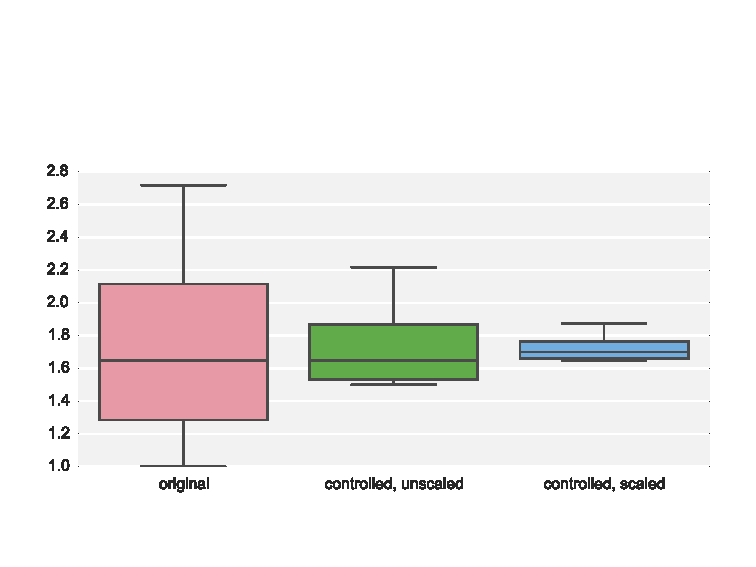
\includegraphics[width=\textwidth]{control-variate.pdf}
% \end{figure}

% end of main matter

\begin{acknowledgements}
The author is grateful to the author, for he is his own eternal flame of inspiration.
\end{acknowledgements}

\appendix
\chapter{Figures}
\label{App:journalcodes}

%BACKMATTER SEE DOCUMENTATION
\backmatter  % references, restarts sample

\printbibliography

\end{document}
